%%%%%%%%%%%%%%%%%%%%%%%%%%%%%%%%%%%%%%%%%
% University of Hong Kong Masters/Doctoral Thesis 
% LaTeX Template
% Version 3.1 (28/03/2023)
% 
% Version 3 modification by:
% Nan Meng (u3003637@connect.hku.hk)
%
% Version 2.x major modifications by:
% Vel (vel@latextemplates.com)
% 
% This template is based on the template by:
% Steve Gunn (http://users.ecs.soton.ac.uk/srg/softwaretools/document/templates/)
% Sunil Patel (http://www.sunilpatel.co.uk/thesis-template/)
% Johannes Böttcher (http://www.latextemplates.com/template/masters-doctoral-thesis)
%
% Template license:
% CC BY-NC-ND 4.0 (https://creativecommons.org/licenses/by-nc-nd/4.0/)
%
% Author:  Lei XIA
% Contact: brianleixia@connect.hku.hk
%
%%%%%%%%%%%%%%%%%%%%%%%%%%%%%%%%%%%%%%%%%


%----------------------------------------------------------------------------------------
%	PACKAGES AND OTHER DOCUMENT CONFIGURATIONS
%----------------------------------------------------------------------------------------

\documentclass[
12pt, % The default document font size, options: 10pt, 11pt, 12pt
%oneside, % Two side (alternating margins) for binding by default, uncomment to switch to one side
english, % ngerman for German
onehalfspacing, % Single line spacing (singlespacing), alternatives: onehalfspacing or doublespacing
% draft, % Uncomment to enable draft mode (no pictures, no links, overfull hboxes indicated)
% nolistspacing, % If the document is onehalfspacing or doublespacing, uncomment this to set spacing in lists to single
liststotoc, % Uncomment to add the list of figures/tables/etc to the table of contents
%toctotoc, % Uncomment to add the main table of contents to the table of contents
parskip, % Uncomment to add space between paragraphs
%nohyperref, % Uncomment to not load the hyperref package
headsepline, % Uncomment to get a line under the header
chapterinoneline, % Uncomment to place the chapter title next to the number on one line
openany
%consistentlayout, % Uncomment to change the layout of the declaration, abstract and acknowledgements pages to match the default layout
]{HKUThesis} % The class file specifying the document structure

\usepackage[utf8]{inputenc} % Required for inputting international characters
\usepackage[T1]{fontenc} % Output font encoding for international characters
\usepackage{fontawesome} % Awesome symbol for usage
\usepackage{wrapfig} % Add enbedded figure in the text
\usepackage{tikz} % Add the signature figure overlap the text
% \usepackage[labelformat=simple]{subcaption} % Add multiple subfigures in a figure environment
% \captionsetup{justification=justified, margin=0pt}
% \renewcommand\thesubfigure{(\Alph{subfigure})} % change the image numbering and reference link to (A),(B),(C), ...... format

\usepackage{mathpazo} % Use the Palatino font by default
\usepackage{bm} % Bold math symbols
%\usepackage[backend=bibtex,style=alphabetic,natbib=true]{biblatex} % Use the bibtex backend with the authoryear citation style (which resembles APA)
\usepackage[backend=bibtex,natbib=true,maxbibnames=99,firstinits=false,sorting=none]{biblatex}

\addbibresource{thesis.bib} % The filename of the bibliography

\usepackage[autostyle=true]{csquotes} % Required to generate language-dependent quotes in the bibliography

\AtBeginEnvironment{enquote}{\itshape} % change the quote words to italics style

\usepackage{rotating} % Required to add rotated big tables

\usepackage[normalem]{ulem} % Required to add dashed underlines

\usepackage[cal=cm]{mathalfa}  % "cm" = Computer Modern (比较规整)

\setlength\parindent{2em}
%----------------------------------------------------------------------------------------
%	MARGIN SETTINGS
%----------------------------------------------------------------------------------------

\geometry{
	paper=a4paper, % Change to letterpaper for US letter
	left=28mm, % Left margin
	right=29mm, % Right margin
	bindingoffset=.5cm, % Binding offset
	top=2.5cm, % Top margin
	bottom=2.5cm, % Bottom margin
	%showframe, % Uncomment to show how the type block is set on the page
}

% Times New Roman font setup
\usepackage{times} % Uncomment this to use Times New Roman font
\usepackage{mathptmx}

\RenewDocumentCommand{\abovechapterskip}{}{\vspace*{-20pt}} % 减小章节标题上方的空间


%----------------------------------------------------------------------------------------
%	THESIS INFORMATION
%----------------------------------------------------------------------------------------

\thesistitle{Topic Guided Multi-faceted Semantic Disentanglement for CTR prediction}
% Thesis title, this is used in the title and abstract, print it elsewhere with \ttitle

\supervisor{Prof. FirstName \textsc{FamilyName}}
% Your supervisor's name, this is used in the title page, print it elsewhere with \supname

\cosupervisor{Prof. FirstName \textsc{FamilyName}}
% Your supervisor's name, this is used in the title page, print it elsewhere with \supname
% \cosupervisor{Prof. Hayden K.-H. \textsc{So}} % Your supervisor's name, this is used in the title page, print it elsewhere with \cosupname

\examiner{}
% Your examiner's name, this is not currently used anywhere in the template, print it elsewhere with \examname

\degree{Master of Science}
% Your degree name, this is used in the title page and abstract, print it elsewhere with \degreename

\author{\textbf{\textsc{Bai} Junhao}, \textbf{\textsc{Long} Qian}, \textbf{\textsc{Yin} Zhiqian}}

% The author name, this is used in the title page and abstract, print it elsewhere with \authorname

\addresses{}
% Your address, this is not currently used anywhere in the template, print it elsewhere with \addressname

\subject{Natural Language Processing}
% Your subject area, this is not currently used anywhere in the template, print it elsewhere with \subjectname

\keywords{CTR Prediction; Disentangled Representation Learning; Topic Model}
% Keywords for your thesis, this is not currently used anywhere in the template, print it elsewhere with \keywordnames

\university{University of Hong Kong}
% Your University's name and URL, this is used in the cover page and abstract, print it elsewhere with \univname

\bsuniversity{HKU}
\msuniversity{HKU}
% Your Bachelor/Master University's name and URL, this is used in the title page and abstract, print it elsewhere with \univname

\department{Department of Computer Science}
% Your department's name and URL, this is used in the title page and abstract, print it elsewhere with \deptname

\group{Laboratory of The Student}
% Your research group's name and URL, this is used in the title page, print it elsewhere with \groupname

\faculty{School of Computing and Data Science}
% Your faculty's name and URL, this is used in the title page and abstract, print it elsewhere with \facname

\AtBeginDocument{
\hypersetup{pdftitle=\ttitle} % Set the PDF's title to your title
\hypersetup{pdfauthor=\authorname} % Set the PDF's author to your name
\hypersetup{pdfkeywords=\keywordnames} % Set the PDF's keywords to your keywords
}
% \AtBeginEnvironment{algorithm}{\setstretch{2}}
\setlength{\algomargin}{1.3ex}


%----------------------------------------------------------------------------------------
%	NEW COMMAND DEFINITION
%----------------------------------------------------------------------------------------
\newcommand{\codestyle}[1]{\colorbox{gray!20}{\darkred{#1}}}

% ======================================================================================== %
%                                        START DOCUMENT
% ======================================================================================== %

\begin{document}

\frontmatter % Use roman page numbering style (i, ii, iii, iv...) for the pre-content pages
\pagestyle{plain} % Default to the plain heading style until the thesis style is called for the body content


%----------------------------------------------------------------------------------------
%	COVER
%----------------------------------------------------------------------------------------

\begin{titlepage}
\addtocounter{page}{-1}
\begin{center}

% \vspace*{.024\textheight}
\begin{center}
    
\includegraphics[width=0.3\textwidth]{Covers/hkulogo.png} % Include the university logo image
\end{center}

% \vspace{0.5cm}
% \textsc{\Large Doctoral Thesis}\\[0.5cm] % Thesis type
\vspace{40pt} % Add some vertical spacing

% University details
\begin{center}
    {The University of Hong Kong}\\[10pt] % University name
    {School of Computing and Data Science}\\[10pt] % Faculty name
    {Department of Computer Science}\\[25pt] % Department name
\end{center}

% \rule[0.4cm]{13cm}{0.1pt}\\% \HRule \\[0.4cm] % Horizontal line
% {\huge \bfseries \ttitle\par}\vspace{0.4cm} % Thesis title
% % \HRule \\[1.5cm] % Horizontal line
% \rule{13cm}{0.1pt}\\ \vspace{1.5cm}
 
% \begin{minipage}[t]{0.4\textwidth}
% \begin{flushleft} \large
% \emph{Author:}\\
% \href{http://#}{\authorname} % Author name - remove the \href bracket to remove the link
% \end{flushleft}
% \end{minipage}
% \begin{minipage}[t]{0.4\textwidth}
% \begin{flushright} \large
% \emph{Supervisor:} \\
% \href{https://www.eee.hku.hk/~elam/}{\supname} \\ % Supervisor name - remove the \href bracket to remove the link
% \emph{Co-Supervisor:} \\
% \href{https://www.eee.hku.hk/~hso/}{\cosupname} % Supervisor name - remove the \href bracket to remove the link 
% \end{flushright}
% \end{minipage}\\[1.6cm]

\vspace{30pt} % Add some vertical spacing
% Course code and dissertation title
\begin{center}
    {COMP7704}\\[10pt] % Course code
    {Dissertation Title}\\ % Dissertation title placeholder
    {Topic Guided Multi-faceted Semantic Disentanglement for CTR prediction}\\[20pt] % Placeholder for the actual title
\end{center}

\vspace{40pt} % Add some vertical spacing

% \large \textit{A thesis submitted in fulfillment of the requirements\\ for the degree of \degreename}\\[0.3cm] % University requirement text
% \textit{in the}\\[0.4cm]
% % \groupname\\
% \deptname\\\facname\\[1.6cm] % Research group name and department name

% Submission details
\begin{center}
    {Submitted in partial fulfillment of the requirements for the admission to\\
    the degree of Master of Science in Computer Science}\\[20pt]
\end{center}

\vspace{20pt} % Add some vertical spacing

% {\large \usdate\today}\\[4cm] % Date
%\includegraphics{Logo} % University/department logo - uncomment to place it

% Author and supervisor details
\begin{center}
    {By\\
    \textbf{\textsc{Bai} Junhao}  ({UID: 3036382909})\\[10pt] 
    \textbf{\textsc{Long} Qian}   ({UID: 3036380559})\\[10pt]
    \textbf{\textsc{Yin} Zhiqian} ({UID: 3036380298})\\[10pt] 
    
    Supervisor: Prof. H.F. Ting\\ % Replace with the supervisor's title and name
    Date of submission: 2025/07/18} % Replace with the submission date
\end{center}

\vfill
\end{center}

\end{titlepage}


% \blankpage
% \addtocounter{page}{-1}


%----------------------------------------------------------------------------------------
%	ABSTRACT PAGE
%----------------------------------------------------------------------------------------


\begin{abstract}
\addchaptertocentry{\abstractname} % Add the abstract to the table of contents
Put Your \emph{Abstract} Here ...

\bigskip
\noindent This latex project is a doctoral thesis template for the University of Hong Kong. The style and design of the entire project closely follow the official guidelines from the Graduate School: \href{https://intraweb.hku.hk/reserved_1/gradsch/PreparingandSubmittingYourThesis.pdf}{\textbf{Preparing and Submitting Your Thesis --- A Guide for MPhil and PhD Students.}} Generally, there is no strict stipulations on the style or format of different components of the thesis, except for the \textbf{Abstract}. According to the detailed regulations [\href{https://intraweb.hku.hk/reserved_1/gradsch/regulations_procedures/format_binding_presentation.pdf}{\textbf{Link}}], the \textbf{Abstract} should be part of the thesis with \uline{no fewer than 200 and no more than 500 words}. The format shall be the same as that of the thesis itself. The front page of each abstract shall contain the statement which includes:
\begin{itemize}
    \item Abstract of thesis entitled ``\dotuline{\hspace{8cm}}''
    \item Submitted by \dotuline{\hspace{10cm}}~
    \item for the degree of \dotuline{\hspace{9.5cm}}~
    \item at the \univname~in (\usdate\today).
\end{itemize}

In addition to the opening of abstract, the abstract \uline{should appear before the title page}. The abstract in this template is \uline{not numbered, or counted in the pagination of the front matter, or listed in the table of contents}. All the requirements are fulfilled in this template.



\end{abstract}


%----------------------------------------------------------------------------------------
%	TITLE PAGE
%----------------------------------------------------------------------------------------
% \pagestyle{empty}
\newpage
\addtocounter{page}{-1}
\begin{center}
\vspace*{2cm}
\huge{ \bf \ttitle}
\end{center}

\vspace{20mm}
\begin{center}
by

\vspace{10mm}
{\bf \authorname}\\
B.S. \textit{\bsunivname} M.S. \textit{\msunivname}
\end{center}

\vspace{30mm}
\begin{center}
A Thesis Submitted in Partial Fulfilment \\
of the Requirements for the Degree of \\
Doctor of Philosophy \\
\vspace{10mm}
at \\
\vspace{10mm}
\univname\\
%February 2015
\monthyeardate\today
\end{center}

%----------------------------------------------------------------------------------------
%	COPYRIGHT PAGE
%----------------------------------------------------------------------------------------

% \newpage
\thispagestyle{empty}
\addtocounter{page}{-1}
\vspace*{\fill}
\scshape \noindent Copyright \copyright 2020, by \authorname \\
\noindent all rights reserved.
\vspace*{\fill}
\newpage
\rm


%----------------------------------------------------------------------------------------
%	DECLARATION PAGE
%----------------------------------------------------------------------------------------

\begin{declaration}
\setcounter{page}{1}
\addchaptertocentry{\authorshipname} % Add the declaration to the table of contents

\vspace{0.6cm}
I, \authorname, declare that this dissertation titled, \enquote{\ttitle}, which is submitted in fulfillment of the requirements for the Degree of Master of Science, represents my own work except where due acknowledgement have been made. I further declared that it has not been previously included in a thesis, dissertation, or report submitted to this University or to any other institution for a degree, diploma or other qualifications.


\vspace{2cm} 
\begin{flushright}
\hfill Signed: \underline{\hspace{5cm}}\\[2em] % This prints a line for the signature
\hfill Date: \underline{\hspace{1.5cm} \usdate\today \hspace{1.5cm}}\\ % This prints a line to write the date
\end{flushright}

% Signature
\begin{tikzpicture}[remember picture,overlay]
\node[xshift=-6cm,yshift=-18cm] at (current page.north east){%
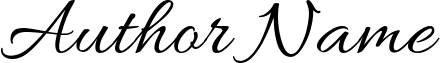
\includegraphics[width=3.6cm]{Figures/signature.png}};
\end{tikzpicture}
\end{declaration}





%----------------------------------------------------------------------------------------
%	QUOTATION PAGE
%----------------------------------------------------------------------------------------

% \newpage
\thispagestyle{empty}
\vspace*{\fill}
\begin{center}
% Font family: ''Calling Angels Personal Use'' from website https://www.dafont.com

\includegraphics[width=0.8\textwidth]{Dedication/dedication.pdf}
\end{center}
\vspace*{\fill}



%----------------------------------------------------------------------------------------
%	ACKNOWLEDGEMENTS
%----------------------------------------------------------------------------------------
\begin{acknowledgements}
\setcounter{page}{2}
\addchaptertocentry{\acknowledgementname} % Add the acknowledgements to the table of contents
\vspace{1cm}


\noindent We would like to thank our supervisor, Professor H.F. Ting, for his guidance and support during the course of this research.
\\[0.4cm]

% \hfill
\begin{flushright}
    \authorname \\
    The University of Hong Kong \\
    \usdate\today
\end{flushright}

\end{acknowledgements}

%----------------------------------------------------------------------------------------
%	LIST OF PUBLICATIONS PAGES
%----------------------------------------------------------------------------------------
% \begin{publications}
\addcontentsline{toc}{chapter}{List of Publications}
\newcommand{\JourConfTitle}[1]{\ul{\emph{#1}}}

% ---------------------------------------------------------------------------
% JOURNALS
% ---------------------------------------------------------------------------

\begin{journals}
\item \textbf{Nan Meng}, Hayden K.-H. So, Xing Sun, and Edmund Y. Lam, ``High-dimens-ional dense residual convolutional neural network for light field reconstruction,'' \JourConfTitle{IEEE Transactions on Pattern Analysis and Machine Intelligence}, October 2019.

\item \textbf{Nan Meng}, Zhou Ge, Tianjiao Zeng, and Edmund Y. Lam, ``LightGAN: a deep generative model for light field reconstruction,'' \JourConfTitle{IEEE Access}, June 2020.

\item \textbf{Nan Meng}, Xing Sun, Hayden K.-H. So, and Edmund Y. Lam, ``Computational light field generation using deep nonparametric Bayesian learning,'' \JourConfTitle{IEEE Access}, vol. 7, pp. 24990--25000, February 2019.

\item \textbf{Nan Meng}, Edmund Y. Lam, Kevin K.-M. Tsia and Hayden K.-H. So, ``Large-scale multi-class image-based cell classification with deep learning,'' \JourConfTitle{IEEE Journal of Biomedical and Health Informatics}, vol. 23, no. 5, pp. 2091--2098, September 2019. 
\end{journals}

% \newpage
% ---------------------------------------------------------------------------
%  CONFERENCES
% ---------------------------------------------------------------------------

\begin{conferences}
\item \textbf{Nan Meng}, Xiaofei Wu, Jianzhuang Liu, and Edmund Y. Lam, ``High-order residual network for light field super-resolution,'' in \JourConfTitle{Association for the Advancement of Artificial Intelligence}, vol. 34, no.7, pp. 11757-11764, 2020.

\item \textbf{Nan Meng}, Tianjiao Zeng, and Edmund Y. Lam, ``Spatial and angular reconstruction of light field based on deep generative networks,'' in \JourConfTitle{IEEE International Conference on Image Processing}, pp. 4659–4663, September 2019.

\item \textbf{Nan Meng}, Tianjiao Zeng, and Edmund Y. Lam, ``Perceptual loss for light field reconstruction in high-dimensional convolutional neural networks,'' in \JourConfTitle{OSA Topical Meeting in Computational Optical Sensing and Imaging}, pp. CW1A.5, June 2019.

\item Edmund Y. Lam, \textbf{Nan Meng}, and Hayden K.H. So, ``Deep convolutional neural network for single-cell image analysis,'' in \JourConfTitle{High-Speed Biomedical Imaging and Spectroscopy: Toward Big Data Instrumentation and Management}, volume 10505 of Proceedings of the SPIE, pp. 105050K, January 2018.

\item \textbf{Nan Meng}, Hayden K.-H. So, and Edmund Y. Lam, ``Computational single-cell classification using deep learning on bright-field and phase images,'' in \JourConfTitle{IAPR Conference on Machine Vision Applications}, pp. 164–167, May 2017.

\item Xing Sun, Zhimin Xu, \textbf{Nan Meng}, Edmund Y. Lam, and Hayden K.-H. So, ``Data-driven light field depth estimation using deep convolutional neural networks,'' in \JourConfTitle{IEEE International Joint Conference on Neural Networks}, pp. 367–374, July 2016.

\item Xing Sun, \textbf{Nan Meng}, Zhimin Xu, Edmund Y. Lam, and Hayden K.-H. So, ``Sparse hierarchical nonparametric Bayesian learning for light field representation and denoising,'' in \JourConfTitle{IEEE International Joint Conference on Neural Networks}, pp. 3272–3279, July 2016.
\end{conferences}

\begin{patents}
\item \textbf{Nan Meng}, Xiaofei Wu, Jianzhuang Liu, ``Image Enhancement and Reconstruction based on Camera Array'', [\emph{under review}]
\end{patents}

\begin{datasets}
\item \textbf{Nan Meng}, Edmund Lam, Tsia, Kevin Kin Man, So, Hayden Kwok-Hay, ``Human somatic label-free bright-field cell images'', IEEE Dataport, 2018. [\darkred{Online}]. Available: \url{http://dx.doi.org/10.21227/H2QW97}. Accessed: Mar. 13, 2019.
\end{datasets}

\end{publications}


%----------------------------------------------------------------------------------------
%	LIST OF CONTENTS/FIGURES/TABLES PAGES
%----------------------------------------------------------------------------------------

\tableofcontents % Prints the main table of contents

\listoffigures % Prints the list of figures

\listoftables % Prints the list of tables

% \listofalgorithms % Prints the list of algorithms
% \addchaptertocentry{\listalgorithmcfname}
%----------------------------------------------------------------------------------------
%	ABBREVIATIONS
%----------------------------------------------------------------------------------------
% \begin{abbreviations}{ll} % Include a list of abbreviations (a table of two columns)

\textbf{ASAP} & \textbf{A}s \textbf{S}oon \textbf{A}s \textbf{P}ossible \\
\textbf{AKA} & \textbf{A}lso \textbf{K}nown \textbf{A}s \\
\textbf{BPFA} & \textbf{B}eta \textbf{P}rocess \textbf{F}actor \textbf{A}nalysis \\
\textbf{CNN} & \textbf{C}onvolutional \textbf{N}eural \textbf{N}etwork \\
\textbf{GAN} & \textbf{G}enerative \textbf{A}dversarial \textbf{N}etwork \\
\textbf{MSE} & \textbf{M}ean \textbf{S}quare \textbf{E}rror \\
\textbf{PSNR} & \textbf{P}eak \textbf{S}ignal-to-\textbf{N}oise \textbf{R}atio \\
\textbf{SSIM} & \textbf{S}tructural \textbf{SIM}ilarity \\

\end{abbreviations}


%----------------------------------------------------------------------------------------
%	SYMBOLS
%----------------------------------------------------------------------------------------
% \begin{symbols}{p{0.15\textwidth}p{0.7\textwidth}l} % Include a list of Symbols (a three column table)

\multicolumn{3}{l}{\symboltitle{Global notations}}\\ \\
$I^\mathrm{SR}$ & super-resolved light field image & --- \\
$I^\mathrm{LR}$ & low-resolution light field image & --- \\
$I^\mathrm{HR}$ & high-resolution light field image & --- \\
$E^\mathrm{SR}$ & super-resolved epipolar plane image & --- \\
$E^\mathrm{HR}$ & high-resolution epipolar plane image & --- \\ \\
% $L$ & light field function & --- \\

\multicolumn{3}{l}{\symboltitle{Chapter~1}}\\ \\
$\theta$, $\phi$ & incoming direction expressed in term of spherical coordinates & rad \\
$\tau$ & time & s (second)\\
$x$,$y$ & spatial coordinates with two-plane parameterization & 1 (uint) \\
$s$,$t$ & angular coordinates with two-plane parameterization & 1 (uint) \\
$P$ & radiance distribution & \si{\watt\per\steradian \square{\metre} \text{\hertz}} \\
$\Omega$ & image plane & --- \\
$\Theta$ & parameters of the multi-layer framework & --- \\
$\gamma_s$, $\gamma_a$ & scaling factors of spatial / angular coordinates & 1 (uint) \\
$\mathcal{L}$ & loss function & --- \\ \\

\multicolumn{3}{l}{\symboltitle{Chapter~2}}\\ \\
$F_0$ & shallow features extracted by a single HConv layer & --- \\
$F_\mathrm{G_d}$ & feature maps extracted by the $d^\mathrm{th}$ HRB of the GRLNet & --- \\
$H_\mathrm{HRB}^\mathrm{n}$ & the operation of the $n^\mathrm{th}$ HRB of the SReNet & --- \\
$H_\mathrm{AGBN}$ & the operation of the proposed aperture group batch normalization algorithm & --- \\
$H_\mathrm{up}$ & upsampling operation on the low-resolution features & --- \\ \\


$\ell_A$ & angular loss & --- \\
$\ell_S$ & spatial perceptual loss & --- \\ 
$\ell_{SA}$ & the weighted combination of $\ell_A$ and $\ell_S$& --- \\
$f$ & the summation of all the feature maps after every activation function of VGG network & --- \\
$g$ & learned mapping between the low-resolution and high-resolution light field images & --- \\ \\


\multicolumn{3}{l}{\symboltitle{Chapter~3}}\\ \\
$x$,$y$ & spatial coordinates with two-plane parameterization & 1 (uint) \\
$s$,$t$ & angular coordinates with two-plane parameterization & 1 (uint) \\
$\gamma_s$, $\gamma_a$ & scaling factors of spatial / angular coordinates & 1 (uint) \\
$\ell_G$ & generator adversarial loss & --- \\
$\phi$ & denotes the mapping of VGG network & --- \\
$\delta$ & nearest neighbor downsampling operator & --- \\
$\kappa$ & a Gaussian blurring kernel with a window size of $7 \times 7$ and standard deviation of 1.2 pixels & --- \\
$\eta$ & additive noise with zero mean and unit standard deviation & --- \\ \\

\end{symbols}


%----------------------------------------------------------------------------------------
%	THESIS CONTENT - CHAPTERS
%----------------------------------------------------------------------------------------

\mainmatter % Begin numeric (1,2,3...) page numbering

\pagestyle{thesis} % Return the page headers back to the "thesis" style

% Include the chapters of the thesis as separate files from the Chapters folder
% Uncomment the lines as you write the chapters

\chapter{Introduction}

\label{chap:introduction}

Click-through rate (CTR) prediction lies at the heart of the online advertising ecosystem and recommendation systems, aiming to estimate a user’s likelihood of clicking on a specific item or advertisement. Accurate CTR predictions enable service providers to generate more relevant and diverse recommendation lists, thereby improving user experience, engagement, and platform revenue. Consequently, CTR prediction has garnered significant attention from both industry professionals and academic researchers.

\begin{figure}[t]
    \centering
    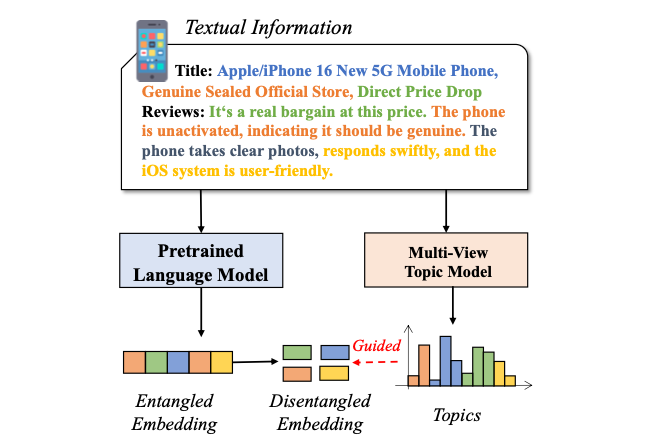
\includegraphics[width=0.9\linewidth]{Figures/Chapter1/figure1.png}
    \caption{Illustration of semantic embedding disentanglement.}
    \label{fig:disentangle}
\end{figure}

Conventional CTR prediction methods typically comprise four main layers: the input layer, embedding layer, interaction layer, and prediction layer. The input layer incorporates a variety of features, including user attributes (e.g., gender, age, occupation, behavior sequences), item characteristics (e.g., category, brand), and contextual information (e.g., interaction location, time). These features are initially processed through the embedding layer to obtain feature embeddings. Subsequently, feature interaction layers, such as Factorization Machines, EulerNet, or KAN, conduct interactions on the feature embeddings. The resulting interacted features are then fed into the prediction layer to estimate the final click probability.

Traditional CTR models primarily rely on structured categorical and numerical features. However, with the rapid advancement of Pretrained Language Models (PLMs), researchers have begun incorporating textual information to enrich semantic understanding and improve prediction accuracy. For instance, CTRL collects textual descriptions of features and encodes them using PLMs to derive semantic embeddings. It employs a contrastive learning strategy to align collaborative signals with these semantic embeddings. Despite the effectiveness of PLMs in extracting semantic features, existing methods typically encode all textual information into a single dense embedding. As illustrated in Figure~\ref{fig:disentangle}, since textual descriptions inherently contain multiple aspects—such as brand, price, quality, and user sentiment—compressing them into a single representation leads to an entangled embedding. This entanglement hinders fine-grained feature interactions, limiting the model’s ability to distinguish between different aspects of user preferences.

Addressing this issue presents two major challenges: 
(1) How can we effectively disentangle and extract meaningful knowledge from textual information? Text descriptions contain rich but interwoven semantic aspects, making it challenging to separate distinct information (e.g., product features, user sentiment, and brand identity) and filter out noise. 
(2) How can we effectively integrate multi-faceted knowledge into the CTR prediction task to extract useful information? Not all extracted textual information is relevant to user decision-making, so aligning it with CTR prediction is crucial for performance improvement.

To address these challenges, we propose \textbf{Multi-faceted Semantic Disentanglement for CTR prediction (MSD-CTR)}. MSD-CTR consists of two components: 
\begin{itemize}
    \item \textbf{Disentangled Semantic Topic Model (DSTopic)} employs a disentangled generative process to capture different aspects of documents using a Disentangled Semantic VAE (DSVAE) and a vocabulary clustering module.
    \item \textbf{Topic Guided Disentangled Representation Learning (TopicDRL)} incorporates the multi-faceted knowledge into CTR prediction, introducing an individual-level alignment loss and an intra-view contrastive loss to guide semantic embedding learning.
\end{itemize}

To evaluate the performance of MSD-CTR, we conduct extensive experiments on four real-world datasets and implement our model based on two foundational CTR methods. The results demonstrate that MSD-CTR outperforms existing CTR models. Additionally, we perform ablation studies and qualitative analyses to validate the effectiveness of the proposed components.

\textbf{Our contributions can be summarized as follows:}
\begin{enumerate}
    \item We investigate text-enhanced CTR methods and analyze the issue of entangled semantic embeddings.
    \item We propose MSD-CTR, a novel framework that disentangles and incorporates multi-faceted knowledge from textual information via DSTopic and TopicDRL modules.
    \item We conduct extensive experiments demonstrating the superior performance of MSD-CTR and validate the contributions of its individual components.
\end{enumerate}



\chapter{Preliminary}

\section{Problem Definition}

Click-through rate (CTR) prediction is a binary classification task. The conventional CTR prediction dataset $\mathcal{D}$ consists of $N$ samples, each represented as a pair $(\mathbf{x}_i, y_i)$, where the label $y_i \in \{0, 1\}$ indicates the user’s click behavior (1 for click, 0 for no click). The input instance is denoted by $\mathbf{x}_i = \{x_{i,1}, x_{i,2}, \cdots, x_{i,m}\}$, where $m$ represents the number of feature fields, and each feature $x_{i,m}$ is a high-dimensional one-hot vector.

In traditional CTR scenarios, a $D$-dimensional embedding layer $\mathcal{E} = \{E_1, E_2, \cdots, E_m\}$ maps the high-dimensional sparse vector $\mathbf{x}_i$ into a low-dimensional dense embedding $\mathbf{e}_i = \{e_{i,1}, e_{i,2}, \cdots, e_{i,m}\}$, where $e_{i,m} \in \mathbb{R}^{D}$, which is more suitable for learning in deep models. The CTR prediction model $f_{\text{CTR}}$ then estimates the click probability $y_i$ based on these embeddings, formulated as:
\[
y_i = f_{\text{CTR}}(e_{i,1}, e_{i,2}, \cdots, e_{i,m}).
\]

\textbf{Text-enhanced CTR prediction:} With the advent of Pretrained Language Models (PLMs), some studies have attempted to incorporate textual information into CTR prediction. Let $t_i$ denote the textual information associated with the sample $(\mathbf{x}_i, y_i)$, which may include the item title, description, and reviews. This textual information is typically encoded by a PLM, formulated as:
\[
\mathbf{t}_i = f_{\text{PLM}}(t_i), \quad \mathbf{t}_i \in \mathbb{R}^{D_{\text{PLM}}},
\]
where $D_{\text{PLM}}$ denotes the dimension of the PLM embedding. The semantic embedding $\mathbf{t}_i$ is then integrated into the CTR model to enhance prediction performance:
\[
y_i = f_{\text{CTR}}(f_{\text{text}}(\mathbf{t}_i), e_{i,1}, e_{i,2}, \cdots, e_{i,m}),
\]
where $f_{\text{text}}$ is a fully connected network that aligns the embedding size to facilitate feature interactions.

Due to the rich information in $t_i$, the encoded semantic embedding $\mathbf{t}_i$ often captures multiple latent aspects, leading to an entangled representation. In this study, we focus on disentangling the entangled semantic embedding $\mathbf{t}_i$ into distinct, meaningful embeddings to enhance interpretability and effectiveness.

\section{Topic Model}

To perform the disentangling task, we employ topic modeling to capture distinct semantic aspects from textual information. A topic model is a statistical approach for discovering hidden semantic structures in a collection of documents. In this study, we treat the textual information of all items as a document corpus, denoted as $\mathcal{T} = \{t_j \mid j \in [1, 2, \cdots, J]\}$, where $J$ is the total number of items. Each document $t_j$ is represented as a Bag-of-Words (BoW) vector $\mathbf{b}_j \in \mathbb{R}^{V}$, where $V$ is the vocabulary size.

The topic model assumes that each document is generated from a mixture of topics (document’s topic distribution), where each topic is characterized by a distribution over words (topic-word distribution). ETM factorizes the topic-word distribution into a topic embedding matrix $\alpha \in \mathbb{R}^{K \times D_{\text{TM}}}$ and a word embedding matrix $\rho \in \mathbb{R}^{V \times D_{\text{TM}}}$, where $K$ is the number of topics and $D_{\text{TM}}$ is the dimensionality of the embeddings. The topic-word distribution matrix $\beta \in \mathbb{R}^{K \times V}$ is computed as:
\[
\beta = \text{Softmax}(\alpha \rho^\top),
\]
where $\beta_{k,v}$ represents the probability of word $v$ given topic $k$.

Let $b_{j,v}$ denote the $v$-th word in document $t_j$. The generative process of $t_j$ follows:
\begin{enumerate}
    \item Draw topic proportions $\theta_j \sim \mathcal{LN}(0, I)$.
    \item For each word $b_{j,v}$ in document $t_j$:
    \begin{enumerate}
        \item Draw a topic assignment $z_{j,v} \sim \text{Cat}(\theta_j)$.
        \item Draw the word $b_{j,v} \sim \text{Cat}(\beta_{z_{j,v}})$.
    \end{enumerate}
\end{enumerate}

Here, $\mathcal{LN}(0, I)$ represents the logistic-normal distribution, which maps a standard Gaussian random variable into the probability simplex, and $\text{Cat}(\cdot)$ denotes the categorical distribution.

% Chapter Template

\chapter{Method} % Main chapter title

\label{ChapterX} % Change X to a consecutive number; for referencing this chapter elsewhere, use \ref{ChapterX}

%----------------------------------------------------------------------------------------
%	SECTION 1
%----------------------------------------------------------------------------------------

\section{Disentangled Semantic Topic Model}

We construct the Disentangled Semantic Topic Model (DSTopic) as a method to extract multi-faceted knowledge from complex and informative textual data. The DSTopic model is specifically designed to address the limitations of traditional topic models, which often rely on the assumption that there is only a single generative process underlying the data. In contrast, DSTopic proposes a disentangled multi-view generative framework, allowing the model to capture and represent different semantic aspects or facets of documents simultaneously. By doing so, DSTopic is able to provide a more comprehensive and structured understanding of the information contained within a collection of texts. However, optimizing the likelihood function in DSTopic directly is generally intractable due to the complexity of the model and the high-dimensional nature of textual data. To address this challenge, we adopt variational inference, which offers an efficient and scalable way to approximate the posterior distributions required for model estimation. In our implementation, DSTopic utilizes a Disentangled Semantic Variational Autoencoder (DSVAE) as its core component, which helps to separate the semantic representations of the data into distinct, meaningful components. In addition, we incorporate a vocabulary clustering module, which further enhances the semantic disentanglement by grouping similar words together. This combined approach enables DSTopic to achieve more accurate and interpretable topic representations, making it a powerful tool for analyzing and understanding large-scale text corpora.


%-----------------------------------
%	SUBSECTION 1
%-----------------------------------
\subsection{Disentangled Generative Process}
\label{chapter:generation}

Unlike traditional topic models that generate documents from a single topic model, DSTopic assumes that each document is generated by topic model with $ H $ distinct views. Each of the $ H $ views is associated with a distinct subset of the vocabulary $\mathcal{V}^{(h)}$. These subsets are disjoint (i.e., they do not share words), ensuring that each view captures an independent semantic aspect of the document. The full vocabulary is reconstructed as the union of all subsets: $ \bigcup_{h=1}^H \mathcal{V}^{(h)} = \mathcal{V} $. 
Accordingly, the $ h $-th view maintains independent topic embeddings $ \alpha^{(h)} \in \mathbb{R}^{\frac{K}{H} \times D_{TM}} $ and word embeddings $ \rho^{(h)} \in \mathbb{R}^{V^{(h)} \times D_{TM}} $, where $ V^{(h)} $ is the size of the corresponding vocabulary set $ \mathcal{V}^{(h)} $. The topic-word distributions of the $ h $-th view, denoted as $ \beta^{(h)} \in \mathbb{R}^{\frac{K}{H} \times V^{(h)}} $, can be computed as: $ \beta^{(h)} = \text{Softmax}(\alpha^{(h)} \rho^{(h)\mathrm{T}}) $. 
Given this framework, the disentangled generative process for document $ t_j $ is as follows:
\begin{enumerate}
    \item For each view $h = 1, \dots, H$:
    \begin{enumerate}
        \item Draw view-aware topic proportions $ \theta_{j}^{(h)} \sim \mathcal{LN}(\mathbf{0}, \mathbf{I}) $ .
    \end{enumerate}
    
    \item For each word $ b_{j,v} $ in the document $ t_j $:
    \begin{enumerate}
        \item Determine the view $ h_{j,v} $ to which the word $ \mathbf{b}_{j,v} $ belongs.
        \item Draw a topic assignment $ \mathbf{z}_{j,v} \sim \text{Cat}(\theta_{j}^{(h_{j,v})}) $.
        \item Draw the word $ b_{j,v} \sim \text{Cat}(\beta_{\mathbf{z}_{j,v}}^{(h_{j,v})}) $.
    \end{enumerate}
\end{enumerate}

In step (1), DSTopic derives the view-aware topic proportions $ \theta_{j}^{(h)} $ for $ h \in [1, 2, \cdots, H] $ from the logistic-normal distribution for the subsequent generation. In step (2), DSTopic first determines the view $ h_{j,v} $ associated with the word $ b_{j,v} $, representing documents as distributions over the topics in $ h_{j,v} $ and drawing a topic assignment for each observed word.


%-----------------------------------
%	SUBSECTION 2
%-----------------------------------

\subsection{Inference and Estimation of the Disentangled Generative Process}
Following the introduction of the disentangled generative process, DSTopic derives the likelihood of optimizing the parameters involved. Specifically, we aim to maximize the marginal likelihood of the documents, formulated as follows:
\begin{align}
    \mathcal{L}(\bm{\alpha}, \bm{\rho}) = \sum_{j=1}^J \sum_{h=1}^H \log p(\mathbf{b}_j^{(h)} | \alpha^{(h)}, \rho^{(h)}),
    \label{eq:likelihood}
\end{align}
where $ \bm{\alpha} = \{\alpha^{(1)}, \alpha^{(2)}, \cdots, \alpha^{(H)}\} $ denotes the set of topic embeddings for all views of the topic model, $ \bm{\rho} = \{\rho^{(1)}, \rho^{(2)}, \cdots, \rho^{(H)}\} $ denotes the vocabulary embedding set for all views, and $ \mathbf{b}_j^{(h)} \in \mathbb{R}^{V^{(h)}} $ represents the Bag-of-Words (BoW) vector under the view $ h $. We introduce a challenging integral over the view-aware topic proportions $ \theta^{(h)} $ and rewrite the probability term as:
\begin{align}
\small
    p(\mathbf{b}_j^{(h)} | \alpha^{(h)} \rho^{(h)}) = \int p(\theta_j^{(h)}) p(\mathbf{b}_j^{(h)} | \theta_j^{(h)}, \alpha^{(h)}, \rho^{(h)}) \, \text{d}\theta_j^{(h)},
\end{align}
The conditional distribution of the BoW vector can be expressed as:
\begin{align}
\small 
    p(\mathbf{b}_j^{(h)} | \theta_j^{(h)}, \alpha^{(h)}, \rho^{(h)}) = \theta_j^{(h)} \beta_j^{(h)} = \theta_j^{(h)} \text{Softmax}(\alpha^{(h)} \rho^{(h)\mathrm{T}}),
\end{align}

However, due to the unknown distribution $ p(\theta_j^{(h)}) $ and the intractable integral, the likelihood in Eq.~\ref{eq:likelihood} remains intractable. To address this issue, ETM \cite{dieng2020topic} introduces a variational distribution $ q(\theta_j; \mathbf{b}_j, \nu) $, where $ \nu $ represents the parameters of the inference network used to derive $ q(\theta_j) $ (noting that there is no disentangled modeling in ETM, so we omit the superscript). However, this variational distribution leverages the BoW vector, neglecting the semantic information present in the document. To address this limitation, we introduce a new variational distribution $ q(\theta_j^{(h)}; \mathbf{t}_j, \nu^{(h)}) $ for a better understanding of the semantic information in the documents. Specifically, $ q(\theta_j^{(h)}; \mathbf{t}_j, \nu^{(h)}) $ is a Gaussian distribution, with its mean and variance derived from an inference network with parameters $ \nu^{(h)} $. This inference network takes the semantic embedding $ \mathbf{t}_j $ of document $ t_j $ as input and outputs the mean and variance of $ \theta_j^{(h)} $.


After introducing this variational distribution, we derive the Evidence Lower Bound (ELBO) to approximate the original likelihood for optimizing both the topic parameters and the variational parameters. The ELBO is formulated as:
\begin{align}
    \mathcal{L}(\bm{\alpha}, \bm{\rho}, \nu) = \sum_{j=1}^J \sum_{h=1}^H &\mathbb{E}_{q(\theta_j^{(h)}; \mathbf{t}_j, \nu^{(h)})} p(\mathbf{b}_j^{(h)} | \theta_j^{(h)}, \alpha^{(h)} \rho^{(h)})  \notag \\
    &- \text{KL}(q(\theta_j^{(h)}; \mathbf{t}_j, \nu^{(h)}) || p(\theta_j^{(h)})),
    \label{eq:elbo}
\end{align}
where $ p(\theta_j^{(h)}) $ is a prior distribution defined as a standard Gaussian distribution $ \mathcal{N}(\mathbf{0}, \mathbf{I}) $, and $\text{KL}(\cdot ||\cdot)$ denotes the KL-divergence.

%-----------------------------------
%	SUBSECTION 3
%-----------------------------------

\subsection{Implementation of Disentangled Generative Process}
In this section, we provide a detailed implementation of the Disentangled Semantic Topic Model (DSTopic), as illustrated in Figure~\ref{fig:architecture}. The implementation consists of two core modules: Vocabulary Clustering and Disentangled Semantic VAE (DSVAE).

\noindent \textbf{(1) Vocabulary Clustering} aims to partition the original vocabulary set into multiple sub-vocabulary sets. We introduce $H$ view embeddings, denoted by $\gamma \in \mathbb{R}^{H \times D_{TM}}$, and compute matching scores between views and words using cosine similarity  $\mathbf{S}' = \rho / |\rho| \left(\gamma /|\gamma|\right)^{\mathrm{T}}$,
%$\mathbf{S}' = \frac{\rho}{|\rho|} \left(\frac{\gamma}{|\gamma|}\right)^{\mathrm{T}}$,
where $\mathbf{S}' \in \mathbb{R}^{V \times H}$ denotes the similarity matrix between views and words, $\gamma$ and $\rho$ denote the embeddings of views and words, respectively, and $|\cdot|$ denotes the L-2 norm of the raw vector of the matrix. To obtain hard cluster labels, we apply the Gumbel-Softmax activation function \cite{jang2016categorical}, formulated as:
\begin{align}
\small
    \mathbf{S} = \frac{\exp(\log \mathbf{S}' - \log(-\log \mathbf{U}))}{\sum_{h=1}^H \exp(\log \mathbf{S}_{\cdot,h}' - \log(-\log \mathbf{U}_{\cdot,h}))} ,
    \label{eq:gumbel}
\end{align}
where $\mathbf{U} \in \mathbb{R}^{V \times H}$ denotes a random matrix sampled from the $\text{Gumbel}(0,1)$ distribution with the same dimensions as the score matrix $\mathbf{S}$, and $\mathbf{S}_{\cdot,h}$ and $\mathbf{U}_{\cdot,h}$ denote the column vectors of matrices $\mathbf{S}$ and $\mathbf{U}$, respectively. After applying Eq.~\ref{eq:gumbel}, each row of $\mathbf{S}$ is a one-hot vector indicating the view to which each word belongs.

\textit{Preventing View Collapse:} During the training of the vocabulary clustering module, we observed the view collapse issue, where a single view contains most words in the vocabulary while other views contain very few words. This collapse hinders further knowledge disentanglement learning. To mitigate this issue, we introduce a variance normalization term, which calculates the variance of the number of words across different views. Specifically, the normalization term $\mathcal{L}_{var}$ is defined as:
\begin{align}
\small
    \mathcal{L}_{var} = \left(\sum_{v=1}^V \mathbf{S}_{v, \cdot} - \frac{\sum_{h=1}^H \sum_{v=1}^V \mathbf{S}_{v, h}}{H}\right)^2 ,
\end{align}
where $\mathbf{S}_{v, \cdot}$ represents the raw vector of matrix $\mathbf{S}$. The first term represents the total number of words belonging to all views, while the second term calculates the mean size of the views.

\noindent \textbf{(2) Disentangled Semantic VAE (DSVAE)} implements the DSTopic using a VAE-based framework, which consists of an Inference Layer (Encoder), a Latent Sampling Layer, and a Generation Layer (Decoder). Specifically, for document $t_j$, as shown in Figure~\ref{fig:architecture}, the \textit{inference layer} aims to extract the view-aware topic embedding $\mathbf{z}_j^{(h)}$ from the semantic embedding $\mathbf{t}_j$, denoted by $\mathbf{z}_j^{(h)} = f_{in}^{(h)}(\mathbf{t}_j)$, where $f_{in}^{(h)}$ is the inference network for view $h$. 

Next, the \textit{latent sampling layer} learns the mean and variance of the view-aware topic proportion $\theta'^{(h)}_j$, denoted by $\theta'^{(h)}_j \sim \mathcal{N}(f_{mean}^{(h)}(\mathbf{z}_j^{(h)}), f_{var}^{(h)}(\mathbf{z}_j^{(h)}))$. To preserve the gradient, we adopt the reparameterization trick following conventional VAE \cite{kingma2013auto} to obtain the sampled $\theta'^{(h)}_j$. A softmax normalization is then applied on $\theta'^{(h)}_j$ to obtain $\theta^{(h)}_j$, ensuring that the probabilities sums to 1. 

Finally, the \textit{generation layer} follows the disentangled generative process presented in Section~\ref{chapter:generation} to reconstruct the view-aware BoW vector $\hat{\mathbf{b}}_j^{(h)}$.

\begin{figure}[t]
    \centering
    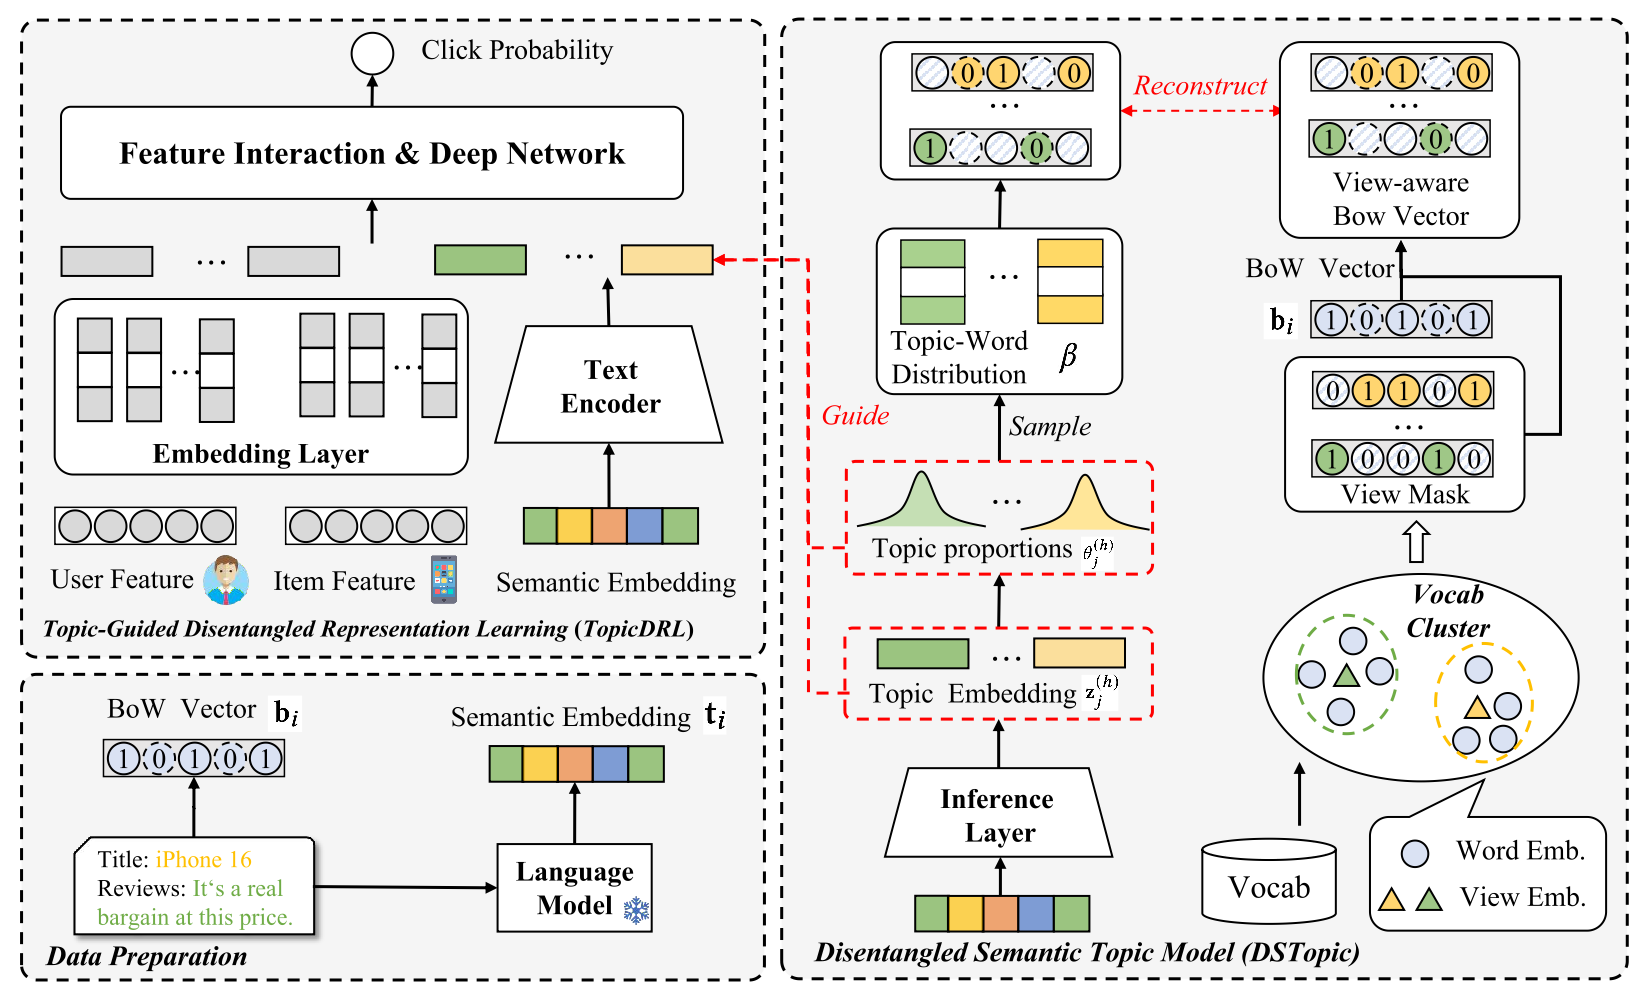
\includegraphics[width=0.9\linewidth]{Figures/Chapter3/fig2.png}
    \caption{Overall architecture of MSD-CTR, which consists of two key components: (1) DSTopic, responsible for extracting disentangled topic representations, and (2) TopicDRL, which integrates these representations into CTR prediction.}
    \label{fig:architecture}
\end{figure}

%----------------------------------------------------------------------------------------
%	SECTION 2
%----------------------------------------------------------------------------------------

\section{Topic Guided Disentangled Representation Learning}

To incorporate multi-faceted knowledge from our disentangled topic model into the CTR prediction task, we initially attempted a straightforward approach by directly integrating the learned view-aware topic embeddings $\mathbf{z}^{(h)}$ into the existing feature set used for prediction. The intuition behind this direct integration was that the topic embeddings, which capture semantic aspects of documents, would naturally enhance the model's ability to predict click-through rates by providing additional contextual information. However, despite this reasonable assumption, this naive operation did not yield the significant performance improvements we expected. In fact, in some experimental settings, directly incorporating these topic embeddings actually introduced negative effects, leading to decreased prediction accuracy compared to baseline models without topic information.

This counterintuitive phenomenon can be attributed to several underlying factors. First and most importantly, the information that is relevant and useful for document generation within the topic model framework is not entirely aligned with the information that is optimal for CTR prediction tasks. While topic models are designed to capture the semantic structure and thematic content of documents, CTR prediction requires understanding user behavior patterns, engagement signals, and factors that influence clicking decisions. These two objectives, though related, operate on different levels of abstraction and require different types of information. Second, directly feeding the topic embeddings $\mathbf{z}^{(h)}$ into the CTR prediction model may inadvertently overlook beneficial information that could be extracted from the topic representations through more sophisticated processing. At the same time, this direct approach may introduce unnecessary noise and irrelevant details that are useful for topic modeling but detrimental to CTR prediction performance.

Given these challenges and the suboptimal results from the direct integration approach, we recognized the need for a more sophisticated method to bridge the gap between topic modeling and CTR prediction. Therefore, we propose the Topic Guided Disentangled Representation Learning (TopicDRL) framework as a refined and more principled alternative to directly using the raw topic embeddings $\mathbf{z}^{(h)}$. The TopicDRL framework is specifically designed to selectively extract and transform the relevant information from the topic embeddings while filtering out noise and irrelevant details. This approach allows us to leverage the multi-faceted knowledge captured by our disentangled topic model in a way that is more aligned with the requirements and objectives of CTR prediction tasks.

TopicDRL encourages disentangled embeddings learning from the semantic embedding $\mathbf{t}_i$, denoted as:
$[\tilde{\mathbf{t}}_i^{(1)}, \tilde{\mathbf{t}}_i^{(2)}, \cdots, \tilde{\mathbf{t}}_i^{(H)}] = f_{text}(\mathbf{t}_i)$
where $\tilde{\mathbf{t}}_i^{(h)} \in \mathbb{R}^D$ represents the disentangled embedding, which has the same dimension as other features in conventional CTR prediction, and $H$ is the number of views, consistent with the number of views in DSTopic. The estimated CTR is computed as:
$
\hat{y}_i = f_{CTR}(\tilde{\mathbf{t}}_i^{(1)}, \tilde{\mathbf{t}}_i^{(2)}, \cdots, \tilde{\mathbf{t}}_i^{(H)}, \mathbf{e}_{i,1}, \mathbf{e}_{i,2}, \cdots, \mathbf{e}_{i,m}).
$



To effectively guide the learning of disentangled embeddings, we introduce two types of alignment losses: an individual-level alignment loss and an intra-view contrastive loss. The \textbf{individual-level alignment loss} $\mathcal{L}_{ind}$ uses the learned multi-view topic embeddings $\mathbf{z}_i^{(h)}$ to supervise the learning of the semantic embeddings $\tilde{\mathbf{t}}_i^{(h)}$. Specifically, $\mathcal{L}_{ind}$ is defined as:
\begin{align}
    \mathcal{L}_{ind} = \sum_{i=1}^N \sum_{h=1}^H |\tilde{\mathbf{t}}_i^{(h)} - f_{tma}(\mathbf{z}_i^{(h)})| ,
\end{align}
where $f_{tma}$ is an adapter implemented by a fully connected network to align the embedding dimensions, $|\cdot|$ is the L-2 norm, and $N$ is the size of the dataset. This loss encourages the semantic embeddings $\tilde{\mathbf{t}}_i^{(h)}$ to focus on shared facet information. Since the disentangled topic embeddings capture different views of knowledge from the textual information, $\mathcal{L}_{ind}$ helps the semantic embeddings $\tilde{\mathbf{t}}_i^{(h)}$ learn in a disentangled embedding space.


Additionally, to normalize the disentangled semantic embeddings learning $\tilde{\mathbf{t}}_i^{(h)}$, TopicDRL introduces an \textbf{intra-view contrastive loss}. This loss assumes that if two items have similar topic distributions in a specific view, their corresponding semantic embeddings should also be similar. Specifically, the intra-view contrastive loss $\mathcal{L}_{int}$ is defined as:
\begin{align}
\small
    \mathcal{L}_{int} = \sum_{h=1}^H \sum_{i=1}^N \frac{\sum_{i'=1}^N a_{i,i'} \exp(\text{sim}(\tilde{\mathbf{t}}_i^{(h)}, \tilde{\mathbf{t}}_{i'}^{(h)}))}{\sum_{i'=1}^N \exp(\text{sim}(\tilde{\mathbf{t}}_i^{(h)}, \tilde{\mathbf{t}}_{i'}^{(h)}))} ,
\end{align}
where $\text{sim}(\cdot, \cdot)$ is a similarity function implemented using cosine similarity, and $a_{i,i'}$ is a weight that estimates the relationship between the textual items $t_i$ and $t_{i'}$, calculated based on the similarity of their topic distributions:
\begin{align}
\small
    a_{i,i'} = \frac{\text{sim}(\mathbf{z}_i^{(h)}, \mathbf{z}_{i'}^{(h)})}{\sum_{i'=1}^N \text{sim}(\mathbf{z}_i^{(h)}, \mathbf{z}_{i'}^{(h)})} ,
\end{align}
Due to the large dataset size $N$, $\mathcal{L}_{int}$ is implemented at the batch level. This loss encourages intra-view relations by pulling semantic embeddings with similar topic distributions closer together while pushing those with dissimilar topic distributions apart.

In addition to the alignment losses, the main CTR prediction loss is defined as a binary cross-entropy loss $\mathcal{L}_{BCE} = - \sum_{i=1}^N [y_i \log \hat{y}_i + (1-y_i)\log (1-\hat{y}_i)]$.
The overall CTR prediction network is trained under the combined CTR loss:
$
\mathcal{L}_{CTR} = \mathcal{L}_{BCE} + \mathcal{L}_{ind} + \mathcal{L}_{int}.
$
\chapter{Experiment} % Main chapter title

\label{ChapterX} % Change X to a consecutive number; for referencing this chapter elsewhere, use \ref{ChapterX}

%----------------------------------------------------------------------------------------
%	SECTION 1
%----------------------------------------------------------------------------------------

\section{Experiment Settings}

\subsection{Datasets and Evaluation Metrics}
\sloppy
We conduct extensive experiments on four large-scale public datasets: Arts\_Crafts\_and\_Sewing (Arts), Grocery\_and\_Gourmet\_Food (Grocery), Office\_Products (Office), and Patio\_Lawn\_and\_Garden (Garden). These datasets include both user interaction data and rich item textual content collected from Amazon \cite{amazon_data}. Each dataset is split into training, validation, and test sets using an 8/1/1 ratio. Following previous work \cite{CTR_work1, CTR_work2}, we employ two widely-used metrics to evaluate performance: AUC and LogLoss. As noted in CTR studies \cite{CTR_study1}, an improvement of 0.001 in AUC (\(\uparrow\)) or Log Loss (\(\downarrow\)) is considered significant, as it can lead to a substantial increase in online revenue.

\subsection{Base CTR Methods and Baselines}
We implement the MSD-CTR based on two foundational CTR methods: DCNv2 \cite{DCNv2} and DeepFM \cite{DeepFM}. Our model is compared against the following competitive methods:
\begin{itemize}
    \item \textbf{Concat:} Directly integrates the semantic embeddings as new features and concatenates them with the traditional CTR features.
    \item \textbf{CTRL:} Employs a contrastive learning strategy to incorporate semantic embeddings \cite{CTRL}.
    \item \textbf{TIGER:} Uses an RQVAE to generate semantic IDs from textual information for subsequent recommendation tasks \cite{TIGER}.
    \item \textbf{MOC:} An enhanced method based on TIGER that utilizes a mixture-of-codes strategy to mitigate information loss \cite{MOC}.
    \item \textbf{VQRec:} A discrete ID-based method that adopts vector-quantized codes using optimized product quantization \cite{VQRec}.
\end{itemize}

\subsection{Implementation Details}
For a fair comparison, we generate \( H \) new features from the semantic embeddings for all baselines (except CTRL) to ensure the same feature count. We set the number of semantic embeddings to 4, i.e., \( H = 4 \). For item textual information, we collect the item title, description, and reviews provided by buyers. We utilize BERT \cite{BERT} as the backbone PLM to obtain semantic embeddings, with the PLM embedding dimension set to \( D_{PLM} = 768 \). For the DSTopic, we set the total number of topics \( K = 100 \) and adopt pre-trained word embeddings generated by BERT, with \( D_{TM} = 768 \). The dimension of the topic embeddings is set to 64. We use the Adam optimizer with a batch size of 2048, a learning rate of 0.001, and a weight decay of \( 1 \times 10^{-6} \) for training DSTopic. For the CTR models, we use the Adam optimizer with a batch size of 2048, a learning rate of 0.001, and a weight decay of \( 1 \times 10^{-6} \). The embedding size for all other experiments is set to 10, i.e., \( D = 10 \). All experiments apply early stopping based on validation AUC with patience of 3. Each experiment is repeated three times with different random initializations. All experiments are conducted on a single NVIDIA GeForce RTX 3090.

%----------------------------------------------------------------------------------------
%	SECTION 2
%----------------------------------------------------------------------------------------

\section{Overall Performance}
\begin{table}[ht]
\centering
\resizebox{\textwidth}{!}{
\begin{tabular}{l|cc|cc|cc|cc}
\toprule
\textbf{Model} & \multicolumn{2}{c|}{\textbf{Arts}} & \multicolumn{2}{c|}{\textbf{Grocery}} & \multicolumn{2}{c|}{\textbf{Office}} & \multicolumn{2}{c}{\textbf{Garden}} \\
\hline
 & \textbf{AUC}$\uparrow$ & \textbf{LogLoss}$\downarrow$ & \textbf{AUC}$\uparrow$ & \textbf{LogLoss}$\downarrow$ & \textbf{AUC}$\uparrow$ & \textbf{LogLoss}$\downarrow$ & \textbf{AUC}$\uparrow$ & \textbf{LogLoss}$\downarrow$ \\
\midrule 
DCNv2 & 0.759727 & 0.405681 & 0.748675 & 0.398848 & 0.755155 & 0.445493 & 0.754589 & 0.463342 \\
Concat & 0.763376 & 0.404141 & 0.74724 & 0.40057 & 0.759956 & 0.443195 & \underline{0.758954} & \underline{0.460755} \\
CTRL & 0.759416 & 0.407308 & 0.744808 & 0.401963 & 0.754862 & 0.446926 & 0.755235 & 0.464106 \\
TIGER & \underline{0.763445} & \underline{0.403398} & \underline{0.750746} & \underline{0.398204} & 0.759498 & 0.442567 & 0.75841 & 0.460965 \\
MOC & 0.762728 & 0.404472 & 0.749354 & 0.399078 & 0.759687 & 0.44234 & 0.757802 & 0.461934 \\
VQRec & 0.763365 & 0.403924 & 0.749727 & 0.398552 & \underline{0.760137} & \underline{0.442207} & 0.758742 & 0.461188 \\
MSD-CTR & \textbf{0.765518} & \textbf{0.402527} & \textbf{0.751367} & \textbf{0.396921} & \textbf{0.761241} & \textbf{0.441938} & \textbf{0.759369} & \textbf{0.459633} \\ 
\bottomrule 
\end{tabular}
}
\caption{Performance comparison of different models. The boldface denotes the highest score and the underline indicates the runner-up of all baselines. Each category contains both AUC and LogLoss metrics.}
\label{tab:performance_comparison}
\end{table}
\begin{table}[ht]
\centering
\resizebox{\textwidth}{!}{
\begin{tabular}{l|ll|ll}
\toprule
\textbf{Variants} & \textbf{DCNv2 AUC$\uparrow$} & \textbf{DCNv2 LogLoss$\downarrow$} & \textbf{DeepFM AUC$\uparrow$} & \textbf{DeepFM LogLoss$\downarrow$} \\ \midrule
MSD-CTR & 0.759369 & 0.459633 & 0.75736 & 0.461959 \\ 
Topic Emb. & 0.759129 & 0.461352 & 0.753654 & 0.466281 \\ 
Topic Prob. & 0.757253 & 0.464738 & 0.756237 & 0.463137 \\ 
w/o ind & 0.758907 & 0.4605 & 0.757183 & 0.462279 \\ 
w/o int & 0.758879 & 0.461624 & 0.756379 & 0.463946 \\ \bottomrule
\end{tabular}
}
\caption{Ablation Study for TopicDRL on Garden.}
\label{tab:ablation_study}
\end{table}


We compare the overall performance of different models, with the results presented in Table \ref{tab:performance_comparison}. From the results, we can draw the following observations:
\begin{itemize}
    \item In most scenarios, incorporating semantic information is beneficial for CTR prediction and leads to performance improvements. However, this is not universally true; in some cases, such as CTRL on the Arts and Grocery datasets, the contrastive learning approach adversely affects the learning of the original features.
    \item Our method outperforms the baselines in most settings, and in other scenarios, it demonstrates competitive performance compared to state-of-the-art (SOTA) methods. These results highlight the effectiveness of disentangling multi-faceted knowledge.
    \item Discrete ID-based methods demonstrate superior performance compared to the naive concat method. However, due to issues such as information loss \cite{MOC} and entangled semantic spaces (as detailed in Section 4.3), these methods perform worse than the proposed approach.
\end{itemize}

%----------------------------------------------------------------------------------------
%	SECTION 3
%----------------------------------------------------------------------------------------

\section{Qualitative Study}
\begin{table}[ht]
\centering
\resizebox{\textwidth}{!}{
\begin{tabular}{l|l|l}
\toprule
\textbf{View ID} & \textbf{Topic Summaries} & \textbf{Topic Words} \\ \midrule
View 0 & Healthy Snacks & coconut, gluten, organic, snack, cookies, crunch, caramel, chocolate, tea \\ 
 & Gift and Special Occasions & friends, delivery, special, occasion, birthday, gifts, beautiful, local, fun, surprise \\ 
 & Beverages and Drinks & milk, espresso, coffee, matcha, smoothie, powder, iced, drink, decaf \\ 
 \hline
View 1 & Product Quality & brand, price, expectations, complaints, review, value, unique \\ 
 & Cooking Essentials & oil, salt, chicken, preparation, spice, blend, texture \\ 
 & Special Ingredients & pumpkin, cream, fat, delicious, artificial, sweeteners, items \\ 
 \hline
View 2 & Dietary Needs & gluten-free, diet, low-sodium, vegan, options, flavorful, energy, ingredients \\ 
 & Snack Preferences & roasted, peanuts, chips, variety, flavors, mix, sweet, savory \\ 
 & Product Variety & selection, packaging, choices, consumer, diversity \\ 
 \hline
View 3 & Cooking and Preparation & baking, recipes, methods, instructions, meals, creative, easy, cooking, flavoring \\ 
 & Ingredient Issues & additives, preservatives, chemicals, health, preferences, quality, taste, satisfaction \\ 
 & Customer Satisfaction & enjoyed, expected, experience, issues, feedback, service, ratings, problems \\ \bottomrule
\end{tabular}
}
\caption{Summary of Learned Topics on Grocery.}
\label{tab:learned_topics}
\end{table}


\subsection{Study on the Learned Topic Model}
We randomly selected learned topics from each view and summarized the keywords using ChatGPT-4o1 for the Grocery dataset. The summaries and corresponding topic words are presented in Table \ref{tab:learned_topics}. Our analysis reveals distinct and disentangled views within the learned topics. For instance, View 0 emphasizes Healthy Snacks and highlights Beverages and Drinks. In contrast, View 1 focuses on Product Quality, addressing consumer expectations and essential cooking ingredients.

\subsection{Visualization of Learned Semantic Embeddings}
We utilize t-SNE \cite{TSNE} to visualize the disentangled topic embeddings $[z^{(1)}_i, z^{(2)}_i, \dots, z^{(H)}_i]$ in DSTopic (a), the learned semantic embeddings $[\tilde{t}^{(1)}_i, \tilde{t}^{(2)}_i, \dots, \tilde{t}^{(H)}_i]$ in TopicDRL (c), and the embeddings from compared methods (b, d-f) using DCNv2, as shown in Figure~\ref{fig:visualization}. We have the following observations:
\begin{itemize}
    \item DSTopic has successfully learned the disentangled multi-view embeddings, which are situated in distinct embedding spaces.
    \item TopicDRL helps CTR prediction by learning disentangled semantic embeddings, demonstrating an improvement over the naive Concat method.
    \item Due to the adoption of RQVAE, TIGER’s first view occupies a different semantic space from the others; however, as a result of information loss, the remaining views become entangled in the same semantic space.
    \item The MoC and VQRec methods fail to learn disentangled semantic embeddings, which limits their overall performance.
\end{itemize}

\chapter{Related Work}

\section{CTR Prediction}

Current click-through rate (CTR) prediction methods can be categorized into two main types: \textit{feature engineering} and \textit{model engineering}.

\subsection{Feature Engineering}

Feature engineering focuses on mining and selecting informative features relevant to CTR prediction. These features include graph features, visual features, textual features, and multimodal features. For example, some methods collect textual descriptions of features, encode the text using pretrained language models (PLMs) to obtain semantic embeddings, and employ alignment loss to align collaborative signals with these embeddings.

Several studies have also focused on filtering out noisy or irrelevant features using automated selection or attention-based methods.

\subsection{Model Engineering}

Model engineering aims to design more effective models to extract information from the input features. This includes developing diverse types of feature interactions, such as Factorization Machines (FM), DeepFM, EulerNet, and KAN.

In addition, many works model user interests—especially long- and short-term interests—based on behavior sequences. These techniques aim to dynamically capture evolving user preferences and improve recommendation quality.

This study falls under the category of feature engineering. Specifically, we mine multi-faceted knowledge from entangled textual information and integrate this knowledge into CTR prediction.

\section{Disentangled Representation Learning}

Disentangled representation learning (DRL) seeks to extract informative and independent factors of variation in data. It has gained significant attention due to its superior explainability.

\subsection{VAE-based Disentanglement}

VAE-based DRL methods can be divided into:
\begin{itemize}
    \item \textbf{Unsupervised approaches}, which re-weight or decompose the evidence lower bound (ELBO) of the VAE to encourage factor separation.
    \item \textbf{Supervised approaches}, which introduce weak supervision signals such as grouping or causal relationships to enforce disentanglement.
\end{itemize}

\subsection{DRL in Recommendation}

DRL for recommendation systems aims to enhance representation learning by separating latent aspects such as:
\begin{itemize}
    \item User interests (e.g., short-term vs. long-term).
    \item Multi-source inputs (e.g., user-item interaction vs. side information).
\end{itemize}

Compared to existing studies, our method focuses on disentangling semantic embeddings from textual side information and using the learned factors to guide CTR prediction.

\section{Topic Model}

Traditional topic models aim to discover latent semantic structures in document collections using probabilistic graphical models (e.g., LDA, dynamic topic models). These models typically infer topic-word and document-topic distributions using methods such as Gibbs sampling or variational inference.

With the success of VAE, neural topic models emerged, which combine the reparameterization trick with BoW-based document representation.

More recently, topic modeling has been extended to PLM-based semantic embeddings. Instead of representing documents as word-count vectors, these methods derive topic distributions from continuous text embeddings, allowing more nuanced topic extraction.

In our work, we propose a disentangled topic model that leverages both BoW structure and semantic embeddings to guide CTR learning.

\section{Qualitative Study}

\subsection{Visualization of Learned Embeddings}

To evaluate the quality of the learned semantic representations, we visualize different models' embeddings using t-SNE. We compare:
\begin{itemize}
    \item Disentangled topic embeddings from \textbf{DSTopic}.
    \item Disentangled semantic embeddings from \textbf{TopicDRL}.
    \item Naive concat embeddings.
    \item Other methods such as \textbf{TIGER}, \textbf{VQRec}, and \textbf{MoC}.
\end{itemize}

\begin{figure}[htbp]
    \centering
    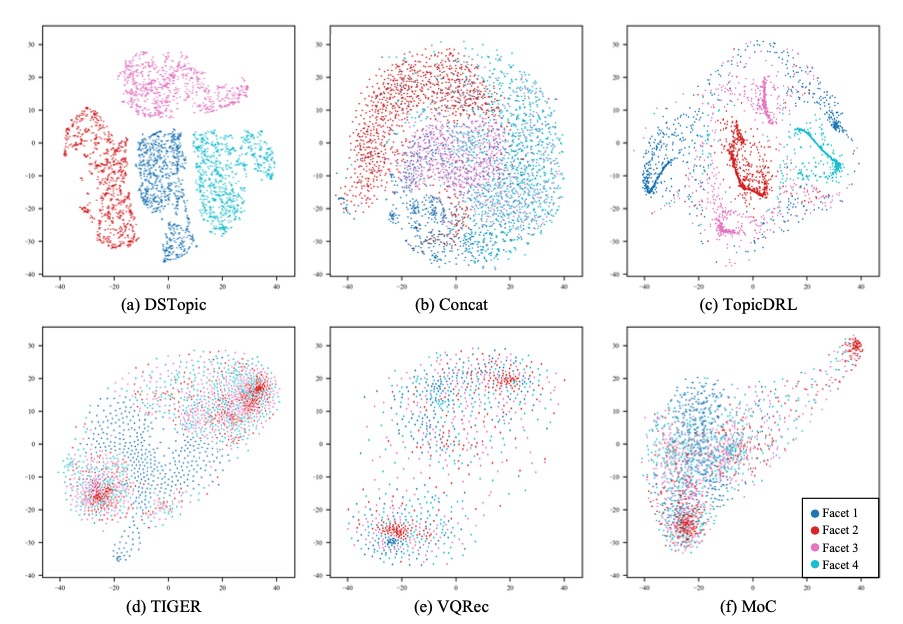
\includegraphics[width=\textwidth]{Figures/Chapter5/fig3.png}
    \caption{Visualization of learned semantic embeddings using DCNv2 on the Garden dataset.}
    \label{fig:tsne}
\end{figure}

We observe that DSTopic and TopicDRL both learn well-separated and interpretable semantic spaces, while other baselines suffer from entanglement or overlap in latent space.

\subsection{Effect of Number of Views}

We vary the number of semantic views $H \in \{1, 2, 4, 6, 8\}$ and compare MSD-CTR against the naive concat method on the Garden dataset. The metrics used are AUC and LogLoss.

\begin{figure}[htbp]
    \centering
    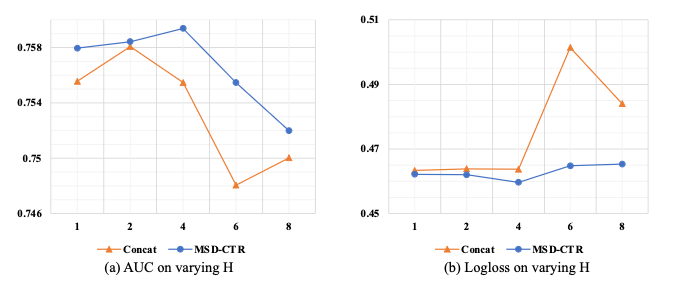
\includegraphics[width=\textwidth]{Figures/Chapter5/fig4.png}
    \caption{Performance comparison on different number of semantic views $H$ for MSD-CTR and Concat.}
    \label{fig:view-ablation}
\end{figure}

Results show that:
\begin{itemize}
    \item MSD-CTR benefits from disentangling semantic knowledge into multiple views.
    \item When $H$ becomes too large, performance drops due to over-fragmentation.
    \item Concat degrades faster due to view overlap and multicollinearity.
\end{itemize}

\chapter{Conclusion}

In this study, we address the critical issue of entangled semantic embeddings, which has been a persistent challenge in click-through rate prediction tasks, and propose \textbf{Multi-faceted Semantic Disentanglement for CTR Prediction (MSD-CTR)} as a comprehensive solution. The main motivation behind our approach stems from the observation that traditional methods often fail to effectively separate and utilize different semantic aspects present in textual data, leading to suboptimal performance in CTR prediction scenarios. Our proposed MSD-CTR framework is designed to tackle this problem through a two-stage approach that first extracts disentangled representations and then effectively incorporates them into the prediction process.

Specifically, MSD-CTR utilizes \textit{DSTopic}, our novel disentangled semantic topic model, to extract and disentangle multi-faceted knowledge from textual information. The \textit{DSTopic} component operates through a carefully designed disentangled topic modeling framework that partitions the vocabulary into distinct subsets, ensuring that each semantic aspect is captured independently without interference from other aspects. This approach allows us to obtain clean, separated representations of different semantic dimensions present in the textual content. Building upon the disentangled representations learned by \textit{DSTopic}, MSD-CTR then employs \textit{TopicDRL} (Topic Guided Disentangled Representation Learning) to effectively incorporate the learned disentangled multi-faceted knowledge into the CTR prediction process. Rather than directly using the topic embeddings, \textit{TopicDRL} introduces carefully designed alignment losses that guide the learning process and ensure that the disentangled semantic information is properly integrated with the prediction objective.

To validate the effectiveness and generalizability of our proposed approach, we implement our method based on two well-established foundational CTR models, allowing us to demonstrate that MSD-CTR can enhance different baseline architectures. We conduct extensive experiments on four diverse CTR datasets that represent different domains and characteristics, ensuring comprehensive evaluation across various scenarios. The experimental results consistently demonstrate the effectiveness of the proposed method, showing significant improvements over baseline models and competing approaches across all tested datasets and base models. Furthermore, to provide deeper insights into the working mechanisms of our approach, we perform comprehensive qualitative and ablation studies. The qualitative studies validate the disentanglement capability of our method by examining the learned semantic aspects and demonstrating their interpretability and distinctiveness. The ablation studies systematically assess the impact of different components of MSD-CTR, including the contribution of \textit{DSTopic}, \textit{TopicDRL}, and various design choices within these modules, providing clear evidence of each component's importance to the overall performance improvement.

%----------------------------------------------------------------------------------------
%	THESIS CONTENT - APPENDICES
%----------------------------------------------------------------------------------------

\appendix % Cue to tell LaTeX that the following "chapters" are Appendices

% Include the appendices of the thesis as separate files from the Appendices folder
% Uncomment the lines as you write the Appendices

% Appendix A

\chapter{Appendix} % Main appendix title
\label{AppendixA} % For referencing this appendix elsewhere, use \ref{AppendixA}
The appendix is usually used to provide some supplementary materials for the publications. For example, some experimental results, network architecture, detailed experimental settings or proving of the theories. You can have more than one appendices to provide the materials for different uses.

% Appendix Template

\chapter{Appendix Title Here} % Main appendix title

\label{AppendixX} % Change X to a consecutive letter; for referencing this appendix elsewhere, use \ref{AppendixX}

Write your Appendix content here.
% Appendix Template

\chapter{Appendix Title Here} % Main appendix title

\label{AppendixX} % Change X to a consecutive letter; for referencing this appendix elsewhere, use \ref{AppendixX}

Write your Appendix content here.


%----------------------------------------------------------------------------------------
%	BIBLIOGRAPHY
%----------------------------------------------------------------------------------------

\nocite{*}
\printbibliography[heading=bibintoc]

%----------------------------------------------------------------------------------------

\end{document}